\begin{exercises} 

\item \label{Ez:10.4.0}   Let $f$ be the function defined by $f(x,y) = x^{1/3}y^{1/3}$, whose graph is shown in Figure \ref{F:10.4.Not_diff}.
\begin{figure}[h]
\begin{center}
%\resizebox{!}{2.5in}{\includegraphics[trim=0cm 0.25cm 0.1cm 1.5cm,clip]{figures/10_4_Not_diff}}
  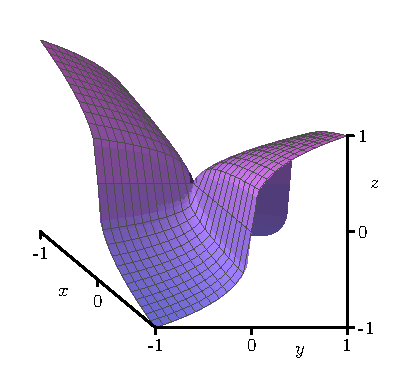
\includegraphics{figures/fig_10_4_not_diff.eps}
\end{center}
\caption{The surface for $f(x,y) = x^{1/3}y^{1/3}$.}
\label{F:10.4.Not_diff}
\end{figure}
    \ba
    \item Determine
    \[\lim_{h \to 0} \frac{f(0+h,0)-f(0,0)}{h}.\]
    What does this limit tell us about $f_x(0,0)$?

    \item Note that $f(x,y)=f(y,x)$, and this symmetry implies that $f_x(0,0) = f_y(0,0)$. So both partial derivatives of $f$ exist at $(0,0)$. A picture of the surface defined by $f$ near $(0,0)$ is shown in Figure \ref{F:10.4.Not_diff}. Based on this picture, do you think $f$ is locally linear at $(0,0)$? Why?

%crop graphics in animate trim=<left> <bottom> <right> <top> (add clip with \includegraphics)

    \item Show that the curve where $x=y$ on the surface defined by $f$ is not differentiable at 0. What does this tell us about the local linearity of $f$ at $(0,0)$?

    \item Is the function $f$ defined by $f(x,y) = \frac{x^2}{y^2+1}$ locally linear at $(0,0)$? Why or why not?

    \ea

\begin{exerciseSolution}
    \ba
    \item With $f(x,y) = x^{1/3}y^{1/3}$ we have 
    \[f_x(0,0) = \lim_{h \to 0} \frac{f(0+h,0)-f(0,0)}{h} = \lim_{h \to 0} \frac{(h^{1/3})(0)-0}{h} = 0.\]

    \item The graph of $f$ seems to indicate some kind of sharp fold in the surface around the point $(0,0)$, so it appears that $f$ is not locally linear at $(0,0)$.

    \item Wen $x=y$ $f$ has the form $f(x,x) = x^{2/3}$. Now
\[\frac{d f(x,x)}{dx}\biggm|_{x=0} = \lim_{h \to 0} \frac{(0+h)^{2/3} - 0}{h} = \lim_{h \to 0} \frac{h^{2/3}}{h} = \lim_{h \to 0} \frac{1}{h^{1/3}}\]
is undefined. Since $f$ does not have a derivative at $(0,0)$ along the path $y=x$, it follows that $f$ defined by $f(x,y) = x^{1/3}y^{1/3}$ is not locally linear at $(0,0)$. Note that neither $f_x$ nor $f_y$ is continuous at $(0,0)$.

    \item For $f(x,y) = \frac{x^2}{y^2+1}$ we have 
\[f_x(x,y) = \frac{2x(y^2+1)}{(y^2+1)^2} \ \text{ and } \ f_y(x,y) = \frac{-2x^2y}{(y^2+1)^2},\]
both of which are continuous around $(0,0)$. So $f$ is locally linear at $(0,0)$. 

    \ea
\end{exerciseSolution}

\item \label{Ez:10.4.1}   Let $g$ be a function that is differentiable at $(-2,5)$ and suppose that its tangent plane at this point is given by $z = -7 + 4(x+2) - 3(y-5)$.				
    \ba
   	\item Determine the values of $g(-2,5)$, $g_x(-2,5)$, and $g_y(-2,5)$.  Write one sentence to explain your thinking.
	\item Estimate the value of $g(-1.8, 4.7)$.  Clearly show your work and thinking.
	\item Given changes of $dx = -0.34$ and $dy = 0.21$, estimate the corresponding change in $g$ that is given by its differential, $dg$.
	\item Suppose that another function $h$ is also differentiable at $(-2,5)$, but that its tangent plane at $(-2,5)$ is given by $3x + 2y - 4z = 9.$  Determine the values of $h(-2,5)$, $h_x(-2,5)$, and $h_y(-2,5)$, and then estimate the value of $h(-1.8, 4.7)$.  Clearly show your work and thinking.
    \ea

\begin{exerciseSolution}
    \ba
   	\item Since the equation of the plane tangent to $g$ at $(-2,5)$ is 
\[L(x,y) = g(-2,5) + g_2(-2,5)(x+2) + g_y(-2,5)(y-5) = -7 + 4(x+2) - 3(y-5)\]
we see that  
\[g(-2,5) = -7, \ g_x(-2,5) = 4, \ \text{ and } \ g_y(-2,5) = -3.\]
	\item The tangent plane approximates the graph of the surface near the point of tangency, so
\[L(x,y) = -7 + 4(x+2) - 3(y-5) \approx g(x,y)\]
when $(x,y)$ is close to $(-2,5)$. Thus,
\[g(-1.8,4.7) \approx L(-1.8,4.7) = -7 + 4(-0.2) - 3(-0.3) = -6.9.\]
	\item The differential $dg$ has the form 
\[dg = g_x(x_0, y_0)dx + g_y(x_0, y_0)dy.\]
In this case, $(x_0, y_0) = (-2,5)$, $dx = -0.34$, and $dy = 0.21$, so
\[dg = 4(-0.34) - 3(0.21) = -1.99.\]
	\item Since the tangent plane $z = \frac{1}{4}(3x+2y-9)$ to $h$ at $(-2,5)$ intersects the graph of $h$ at $(-2,5)$, it follows that $h(-2,5) = \frac{1}{4}(3(-2)+2(5)-9) = -\frac{5}{4} = -1.25$. We also have $h_x(-2,5) = 3$ and $h_y(-2,5) = 2$. Then
\[h(-1.8, 4.7) \approx \frac{1}{4}(3(-1.8)+2(5)-9) = -1.1.\]

    \ea
\end{exerciseSolution}

\item \label{Ez:10.4.2}   In the following questions, we determine and apply the linearization for several different functions.				
    \ba
   	\item Find the linearization $L(x,y)$ for the function $f$ defined by $f(x,y) = \cos(x)(2e^{2y}+e^{-2y})$
at the point $(x_0,y_0) = (0,0)$.  Hence use the linearization to estimate
the value of $f(0.1, 0.2)$.  Compare your estimate to the actual value of $f(0.1, 0.2)$.

	\item The Heat Index, $I$, (measured in apparent degrees F) is a function of the actual temperature $T$ outside (in degrees F) and the relative humidity $H$ (measured as a percentage).  A portion of the table which gives values for this function, $I(T,H)$, is provided below:
\begin{center}
\begin{tabular}{|l||r|r|r|r|} \hline
\emph{T} $\downarrow \backslash$ \emph{H} $\rightarrow$ & 70 &	75 & 80 &	85  \\ \hhline{|=|=|=|=|=|}
90 & 106 & 109 & 112 & 115  \\ \hline
92 & 112 & 115 & 119 & 123  \\ \hline
94 & 118 & 122 & 127 & 132  \\ \hline
96 & 125 & 130 & 135 & 141  \\ \hline
\end{tabular}
\end{center}
Suppose you are given that $I_T(94,75) = 3.75$ and $I_H(94,75) = 0.9$.  Use this given information and one other value from the table to estimate the value of $I(93.1,77)$ using the linearization at $(94,75)$.  Using proper terminology and notation, explain your work and thinking.
	\item Just as we can find a local linearization for a differentiable function of two variables, we can do so for functions of three or more variables.  By extending the concept of the local linearization from two to three variables, find the linearization of the function $h(x,y,z) =
  e^{2x}(y+z^2)$ at the point $(x_0,y_0,z_0) = (0, 1, -2)$.  Then, use the
  linearization to estimate the value of $h(-0.1, 0.9, -1.8)$.
    \ea

\begin{exerciseSolution}
    \ba
   	\item If $f(x,y) = \cos(x)(2e^{2y}+e^{-2y})$, then
\[f_x(x,y) = -\sin(x)(2e^{2y}+e^{-2y}) \ \text{ and } \ f_y(x,y) = \cos(x)\left(4e^{2y} - 2e^{-2y}\right).\]
So
\[f_x(0,0) = 0 \ \text{ and } \ f_y(0,0) = 2.\]
So the linearization of $f$ at $(0,0)$ is 
\[L(x,y) = f(0,0) + f_x(0,0)(x-0)+f_y(0,0)(y-0) = 3+2y.\]
Then
\[f(0.1,0.2) \approx L(0.1,0.2) = 3.4.\]
By calculator, the value of $f(0.1,0.2)$ is approximately $3.635714815$, so our approximation with the linearization is off by about $0.23$.

	\item Since $I(94,75) = 122$, the linearization of $I$ at $(94,75)$ is 
\[L(x,y) = I(94,75) + I_T(94,75)(T-94) + I_H(94,75)(H-75) = 122 + 3.75(T-94) + 0.9(H-75).\]
Thus,
\[I(93.1,77) \approx L(93.1,77) = 122 + 3.75(-0.9) + 0.9(2) = 120.425.\]

	\item The linearization of $h$ at $(x_0,y_0,z_0)$ will be 
\[L(x,y,z) = h(x_0,y_0,z_0) + h_x(x_0,y_0,z_0)(x-x_0) + h_y(x_0,y_0,z_0)(y-y_0) + h_z(x_0,y_0,z_0)(z-z_0).\]
For our function $h$ we have 
\[h_x(x,y,z) = 2e^{2x}(y+z^2), \ h_y(x,y,z) = e^{2x}, \ \text{ and } \ h_z(x,y,z) = e^{2x}(2z).\]
So
\[h_x(0,1,-2) = 10, \ h_y(0,1,-2) = 1, \ \text{ and } \ h_z(0,1,-2) = -4\]
and the linearization of $h$ at $(0,1,-2)$ is 
\[L(x,y,z) = 5 + 10x + (y-1) - 4(z+2).\]
Thus,
\[h(-0.1, 0.9, -1.8) \approx L(-0.1, 0.9, -1.8) = 3.1.\]
	\ea
	
\end{exerciseSolution}

\item \label{Ez:10.4.3}   In the following questions, we investigate two different applied settings using the differential.

\ba

	\item Let $f$ represent the vertical displacement in centimeters from the rest position of a string (like a guitar string) as a function of the distance $x$ in centimeters from the fixed left end of the string and $y$ the time in seconds after the string has been plucked.\footnote{An interesting video of this can be seen at \url{https://www.youtube.com/watch?v=TKF6nFzpHBUA}.} A simple model for $f$ could be
\[f(x,y) = \cos(x)\sin(2y).\]
Use the differential to approximate how much more this vibrating string is vertically displaced from its position at $(a,b) = \left(\frac{\pi}{4}, \frac{\pi}{3} \right)$ if we decrease $a$ by $0.01$ cm and increase the time by $0.1$ seconds. Compare to the value of $f$ at the point $\left(\frac{\pi}{4}-0.01, \frac{\pi}{3}+0.1\right)$.

   	\item Resistors used in electrical circuits have colored bands painted
  on them to indicate the amount of resistance and the possible error
  in the resistance.  When three resistors, whose resistances are
  $R_1$, $R_2$, and $R_3$, are connected in parallel, the total
  resistance $R$ is given by
  $$
  \frac1R = \frac1{R_1} + \frac1{R_2} + \frac1{R_3}.
  $$
  Suppose that the resistances are $R_1=25\Omega$, $R_2=40\Omega$, and
  $R_3=50\Omega$.  Find the total resistance $R$.

  If you know each of $R_1$, $R_2$, and $R_3$ with a possible error of
  $0.5$\%, estimate the maximum error in your calculation of $R$.

\ea

\begin{exerciseSolution}
\ba
\item First note that
\[\frac{\partial f}{\partial x} = -\sin(x)\sin(2y) \ \ \text{ and } \ \ \frac{\partial f}{\partial y} = 2\cos(x)\cos(2y)\]
and
\[f_x\left(\frac{\pi}{4}, \frac{\pi}{3}\right) = -\sin\left(\frac{\pi}{4}\right)\sin\left(\frac{2\pi}{3}\right) = -\frac{\sqrt{6}}{4} \ \ \text{ and } \ \ f_y\left(\frac{\pi}{4}, \frac{\pi}{3}\right) = 2\cos\left(\frac{\pi}{4}\right)\cos\left(\frac{2\pi}{3}\right) = -\frac{\sqrt{2}}{2}.\]

So with $dx = -0.01$ and $dy = 0.1$ we have 
\[df = f_x(a,b)(-0.01) + f_y(a,b)(y-b) = -\frac{\sqrt{6}}{4}(-0.01) - \frac{\sqrt{2}}{2}(0.1) \approx -0.065.\]
So the string is vertically displaced approximately $-0.064$ centimeters from its position at $(a,b)$. Comparing to the exact displacement
\[f(a,b) - f(a-0.01, b+0.1) \approx 0.077,\]
we see that our approximation is off by about $0.01$.

\item The total resistance $R$ satisfies 
\[\frac{1}{R} = \frac{1}{25} + \frac{1}{40} + \frac{1}{50} = \frac{17}{200},\]
so 
\[R = \frac{200}{17}.\]
We can write $R$ as 
\[R = \frac{R_1R_2R_3}{R_2R_3+R_1R_3+R_1R_2}.\]
Then
\begin{align*}
R_{R_1}(R_1,R_2,R_3) &= \frac{(R_2R_3+R_1R_3+R_1R_2)(R_2R_3)-R_1R_2R_3(R_3+R_2)}{(R_2R_3+R_1R_3+R_1R_2)^2} \\
R_{R_2}(R_1,R_2,R_3) &= \frac{(R_2R_3+R_1R_3+R_1R_2)(R_1R_3)-R_1R_2R_3(R_3+R_1)}{(R_2R_3+R_1R_3+R_1R_2)^2} \\
R_{R_3}(R_1,R_2,R_3) &= \frac{(R_2R_3+R_1R_3+R_1R_2)(R_1R_2)-R_1R_2R_3(R_2+R_1)}{(R_2R_3+R_1R_3+R_1R_2)^2}.
\end{align*}
This gives us
\begin{align*}
R_{R_1}(25, 40, 50) &= \frac{64}{289} \\
R_{R_2}(25, 40, 50) &= \frac{25}{289}  \\
R_{R_3}(25, 40, 50) &= \frac{16}{289}.
\end{align*}
If $dR_1 = dR_2 = dR_3 = 0.005$, then 
\begin{align*}
dR &= R_{R_1}(25, 40, 50) dR_1 + R_{R_2}(25, 40, 50) dR_2 + R_{R_3}(25, 40, 50) dR_3 \\
	&= \left(\frac{64}{289} + \frac{25}{289} + \frac{16}{289} \right) (0.005) \\
	&\approx 0.0018.
\end{align*}
So the maximum error in our calculation is about 0.18\%. 

\ea
\end{exerciseSolution}
\end{exercises}
\afterexercises
